\section{Introduction}
	\paragraph{}{
	This chapter will outline the overall system and user interface design of the application. This will include explanations on design decisions made during the project and how the overall design will satisfy the requirements outlined in chapter 3.
	}

\section{System Design}
	\paragraph{}{
	%Intro
	The goal of the system design is to create an extensible and portable application. Any additional core features or aesthetic changes should plug in to the existing system without affecting its current functionality. This can be achieved by applying Martin Fowler's concept of the three principle layers in the design: the presentation layer, representing the user interface, the domain layer, representing the business logic and the data source layer representing communication with another system such as a database.\cite{Fowler}
	}
	\begin{figure}[h]
		\begin{center}
			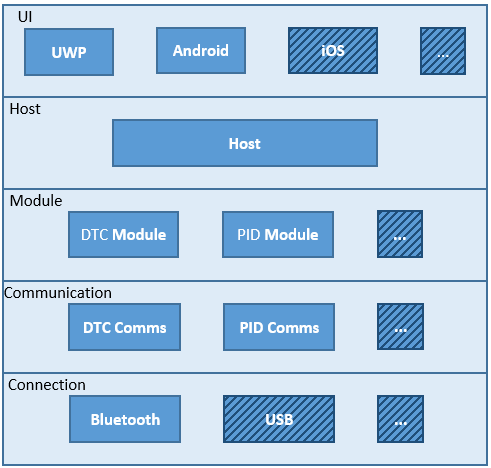
\includegraphics[width=0.5\textwidth]{Architecture.png}
			\caption{System Architecture - Shaded items will not be implemented}
			\label{fig:Architecture}
		\end{center}
	\end{figure}
	\paragraph{}{
	Looking at figure \ref{fig:Architecture}, the UI layer represents the presentation layer, the connection layer represents the data layer and the host, module and communication layers can be combined to represent the domain layer.
	%[EXPLAIN THIS MORE CONCISELY, RE-FACTOR FOLLOWING PARAGRAPHS]		
	}	
	
	\paragraph{}{
	The UI layer represents the user interface and user input handling functionality of the application. Gesture controls, such as swiping, scrolling and pinching are handled and buttons presses are hooked up to the appropriate functionality in the host or module. To port the application to another system, the developer only creates a new UI layer, as the UI is completely abstracted from the core functionality of the system.
	}	
	
	\paragraph{}{
	The host acts as a connection between the core functionality of the application and the UI and user input. The user interface connects to the host, which grants access to the modules that are registered with it. The modules are registered with the host on initialization of the application. This means new modules can be created and added to the application, without requiring a new build.
	}
		
	\begin{figure}[h]
		\begin{lstlisting}
public interface IHost : INotifyPropertyChanged
{
	// List of all Modules associated with the Host
	IList<IModule> Modules { get; }
	
	// The currently selected Module
	IModule CurrentModule { get; set; }
}
		\end{lstlisting}
		\caption{Host Interface}
		\label{code:HostInterface}
	\end{figure}
	
	\paragraph{}{
	The module represents the model in the MVVM pattern and a core function, such as a mode, in the system. The module contains human readable data that is retrieved from the vehicle. In order to obtain this data, the module must send a request to its communication system. The communication system, which is a part of each module, will take this request and convert it into the corresponding command that the ELM327 device and ECU can understand. It will then send this new request to the connection layer and await a response. This response, in the form of raw hexadecimal data, will be converted into a human readable value by the communication system and returned to the module, ready to be displayed or manipulated.
	}
	\begin{figure}[h]
		\begin{lstlisting}
public interface IModule : INotifyPropertyChanged
{
	// The name of the Module
	string Name { get; }
	
	// A list of hints and tips for how to use the Module
	IList<IHelpItem> HelpItems { get; }

	// Initialize the Module
	Task<bool> Initialize();

	// Shut down the Module
	Task<bool> Shutdown(); 
}
		\end{lstlisting}
		\caption{Module Interface}
		\label{code:ModuleInterface}
	\end{figure}
	
	\paragraph{}{
	The connection layer represents the low level communication with the OBDII device, such as the ELM327 device. This layer handles the initialization and configuration of the connected device, as well as error handling, such as when the device is disconnected during a procedure or becomes out of range. All requests and responses are handled in hexadecimal format in this layer, allowing the use of raw data to be abstracted from the other layers.
	%Initialization, Setup of device, Handles raw data
	}
	\begin{figure}[h]
		\begin{lstlisting}
public interface IDataConnection : INotifyPropertyChanged
{	
	bool IsInitialized { get; }

	// Logs the command, response and time for each request
	string CommunicationLog { get; }

	// The status of the connected device
    ConnectionStatus DeviceConnectionStatus { get; set; }

	// The protocol of the current vehicle
	Protocol VehicleProtocol { get; }

	// The current connected device
    IDevice CurrentDevice { get; set; }

	// A list of devices the application can connect to
	Task<IList<IDevice>> GetAvailableDevices();

	// Initialize the connection
	Task<bool> Initialize();	

	// Reset the connection
	Task<bool> Reset();

	// Send a request to the device
    Task<string> SendCommand(string command);
}
		\end{lstlisting}
		\caption{Connection Interface}
		\label{code:ConnectionInterface}
	\end{figure}

\section{UI Design}
	\paragraph{}{
	It was necessary to create a coherent and highly usable user interface for this application, to satisfy the requirements of the project. This would involve creating a shared look and feel for each module in the application, so that when transitioning from one to the other, the user can easily navigate the user interface and find the functions they need to use with no learning curve.
	%Intro - Created using Pencil
	}	
	\paragraph{}{
	This was achieved by creating a UI shell, as seen in figure \ref{fig:UIShell}, with unified controls and look and feel that would be displayed regardless of which module is currently selected. The shell acts as a means to select and view the current module as well as configure the application, such as which device is connected. Inside the shell, there is a view that the current module will occupy. Each module UI will match the color scheme, font and layout of the UI shell.
	%Microsoft UI Guideline?	
	}
	
	\begin{figure}[h]
		\begin{center}
			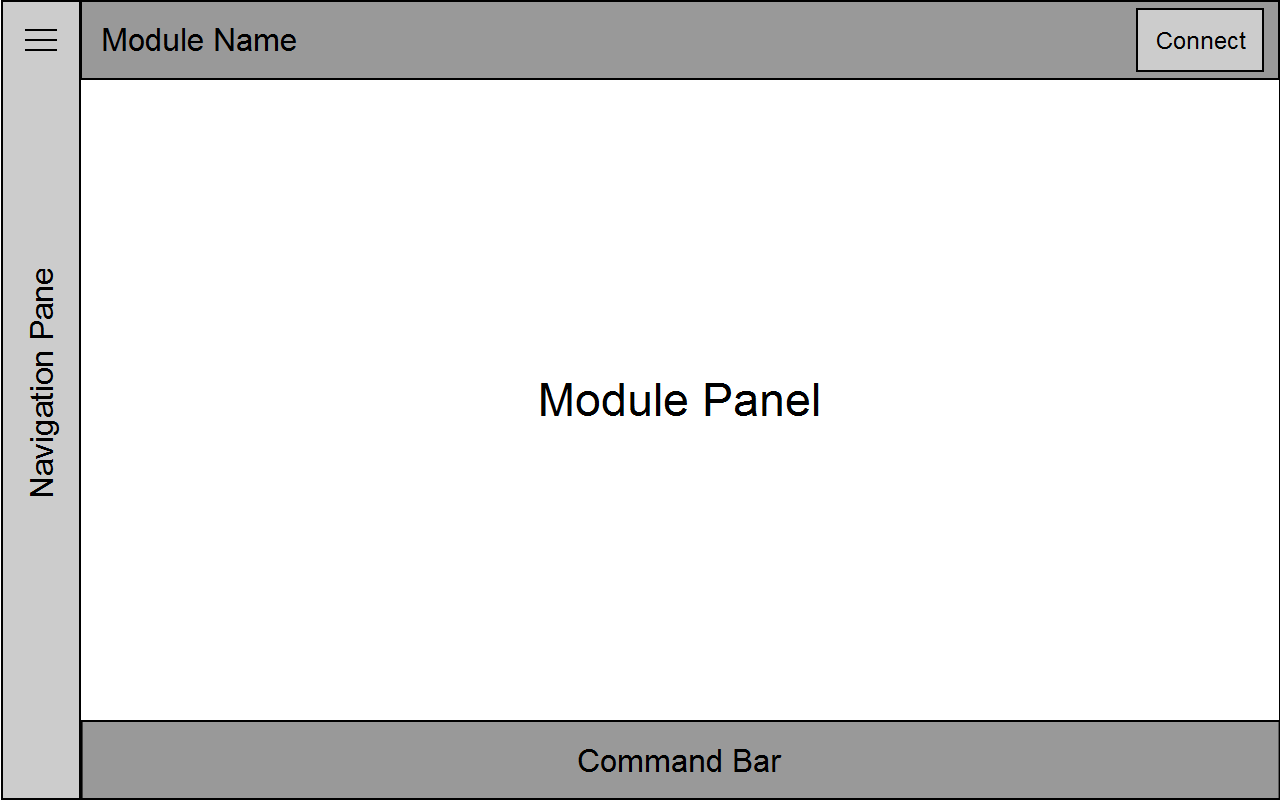
\includegraphics[width=0.5\textwidth]{hostpage.png}
			\caption{UI Shell}
			\label{fig:UIShell}
		\end{center}
	\end{figure}	
	
	\paragraph{}{
	A number of mockups were created for the user interface using an application called Pencil. These were simple wireframes and did not include platform specific UI elements, but instead provide a more abstract view of the overall look and feel of the application. The mockups served as an initial guide when implementing the user interface and as a means of maintaining a coherent and standardised UI. 
	% UI Mockups
	}
	\paragraph{}{
	[XAML with C\#]
	}
	
	\subsection{DTC Module}
		\paragraph{}{						
		% Must display description as well as code, allow the user to clear codes, display additional information, if needed, without interupting flow
		[INTRO]
		}
		\paragraph{}{
		[CODE LIST]
		}
		\paragraph{}{
		[CODE DETAILS]
		% Get more info, without interrupting flow of application. Design chocies include take user to a separate screen, load a modal box, or add a drop down box
		}
		\begin{figure}[h]
			\begin{center}								
				\begin{minipage}{0.49\textwidth}
					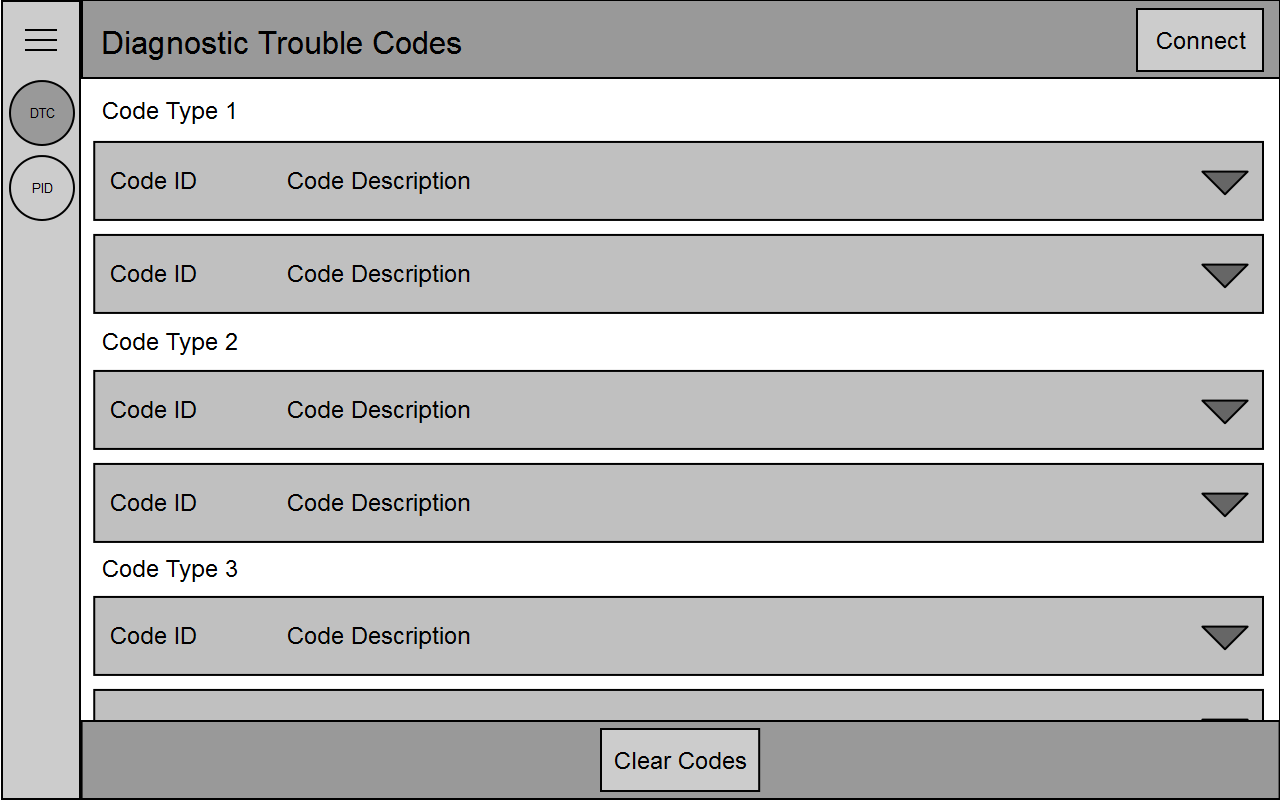
\includegraphics[width=\textwidth]{dtcpage.png}
					\caption{DTC Page}						
					\label{fig:DTCPage1}
				\end{minipage}
				\hfill			
				\begin{minipage}{0.49\textwidth}
					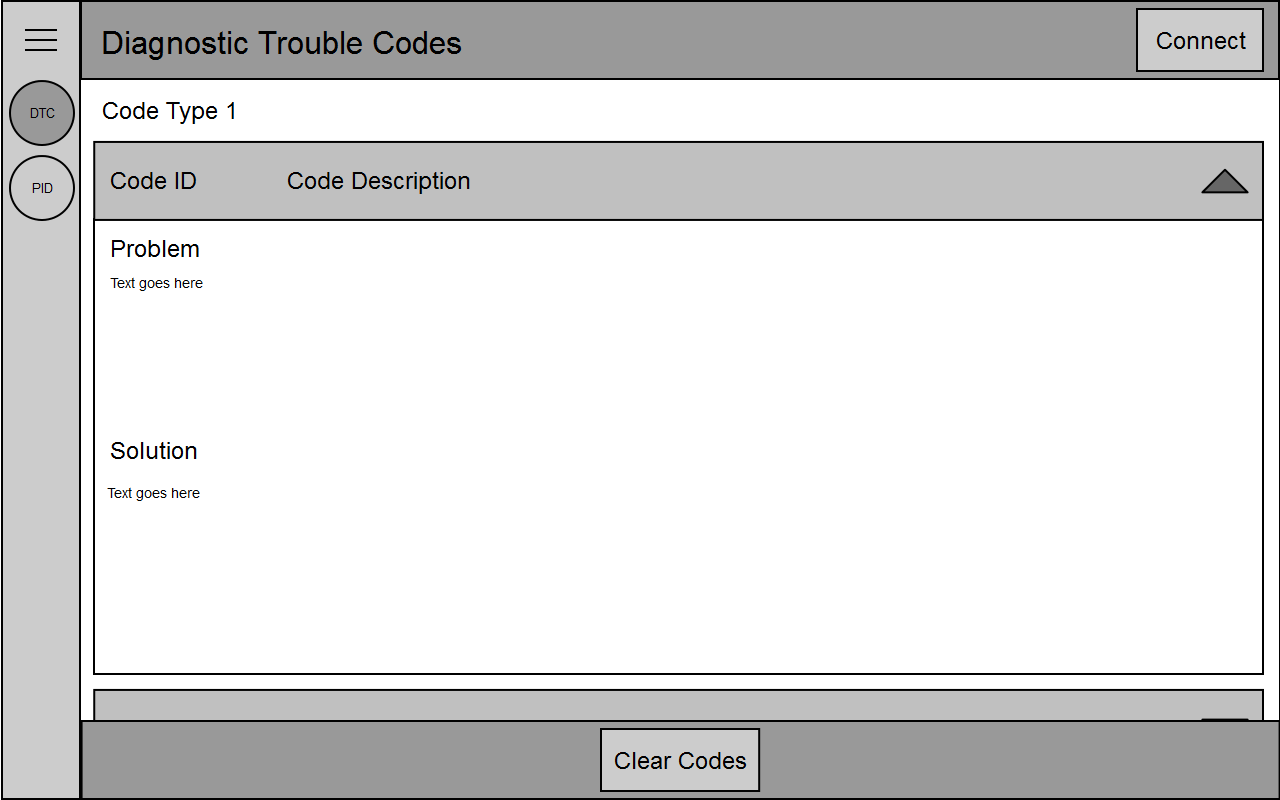
\includegraphics[width=\textwidth]{dtcpage2.png}
					\caption{DTC Page with information}						
					\label{fig:DTCPage2}
				\end{minipage}									
			\end{center}
		\end{figure}
	\newpage
	\subsection{Data Module}
		\paragraph{}{	
		The user interface for the data module consists of two components: data text views and data graph views.  
		% Graphs as well as text, smart graphing, expand and collapse graph, fullscreen graph
		}
		\paragraph{}{
		In the data module, the text views show the current data value in text format, enabling the user to see the current state of the vehicle at a glance. During the design process, displaying the current value on a dial was considered, as seen in the similar applications. This would create a match between the system and real world, as this is how these values are displayed on the dashboard of their car.
		%[TEXT VIEWS] - Considered dials like similar applications
		}
		\paragraph{}{
		However, this approach would lead to the user interface becoming cluttered if a large number of items were on-screen, leading to decreased usability. Instead, a list format was considered, as seen on the left side of figure \ref{fig:DataPage1}. This allowed for a minimalist design that would remain consistent when the number of available pids increased. This approach was eventually selected, as it achieved the same goal of displaying the current value for a pid in a more simplistic and user friendly manner.
		}
		\paragraph{}{
		The key aspect of the data module user interface is the graphing of data values. By graphing the data, the user can track the values throughout the history of current session. 
\\		
		It also provides a more visual representation for the data, allowing the user to identify the maximum, minimum and average values at a glance. As a user may only want to view one particular graph or a subset of graphs, the design allows for user to minimise certain graphs and to set one graph to fullscreen mode for more detailed viewing, as seen in figure \ref{fig:DataPage2}.
		%[GRAPH VIEWS]
		% Smart graphing, the design allow for users to minimise graphs and expand them to full screen
		}
		\paragraph{}{
		The user may want to move forwards and backwards through the data samples that have been collected, to find a particular value. To accommodate this, the design contains controls in the command bar. These include a play and pause button, to start and stop gathering, as well as skip buttons to move through the samples.
		%[CONTROLS]
		}
		\begin{figure}[h]
			\begin{center}								
				\begin{minipage}{0.49\textwidth}
					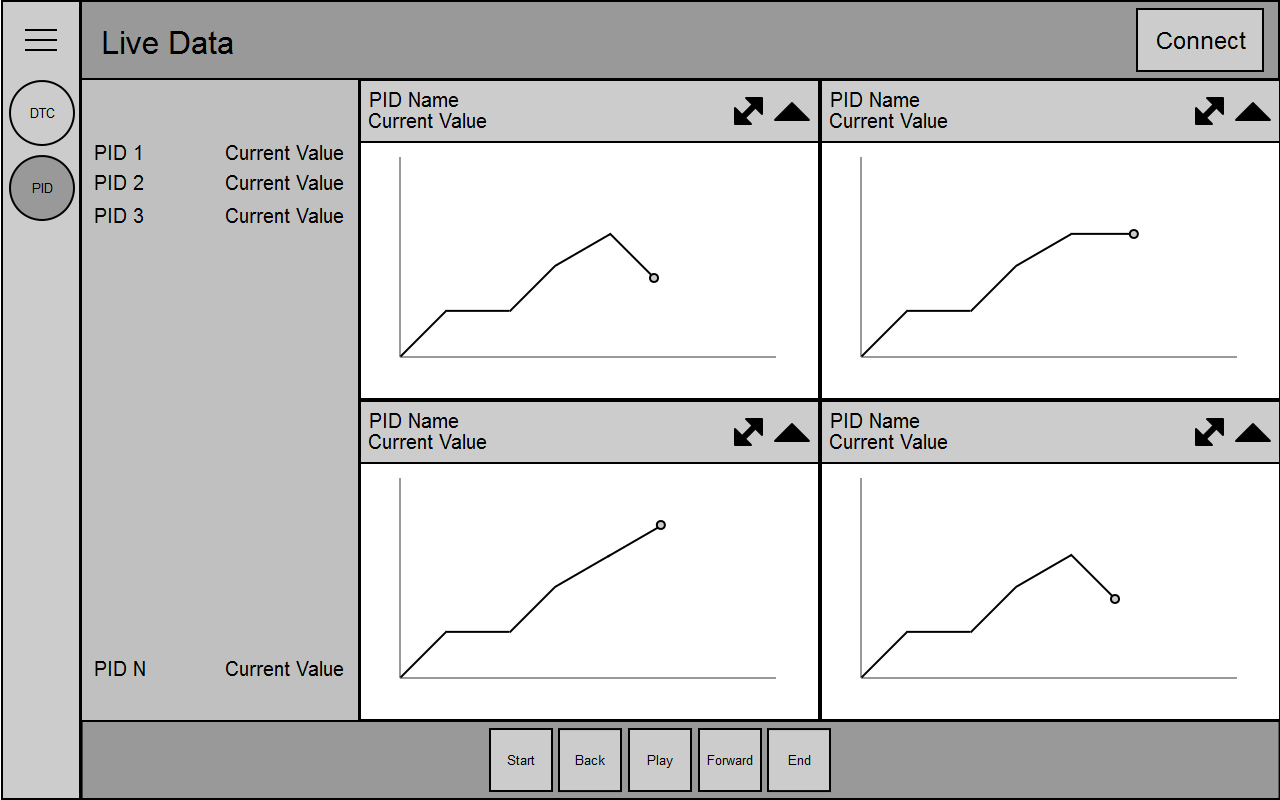
\includegraphics[width=\textwidth]{pidpage.png}
					\caption{Data Page - Graphs Expanded}						
					\label{fig:DataPage1}
				\end{minipage}
				\hfill			
				\begin{minipage}{0.49\textwidth}
					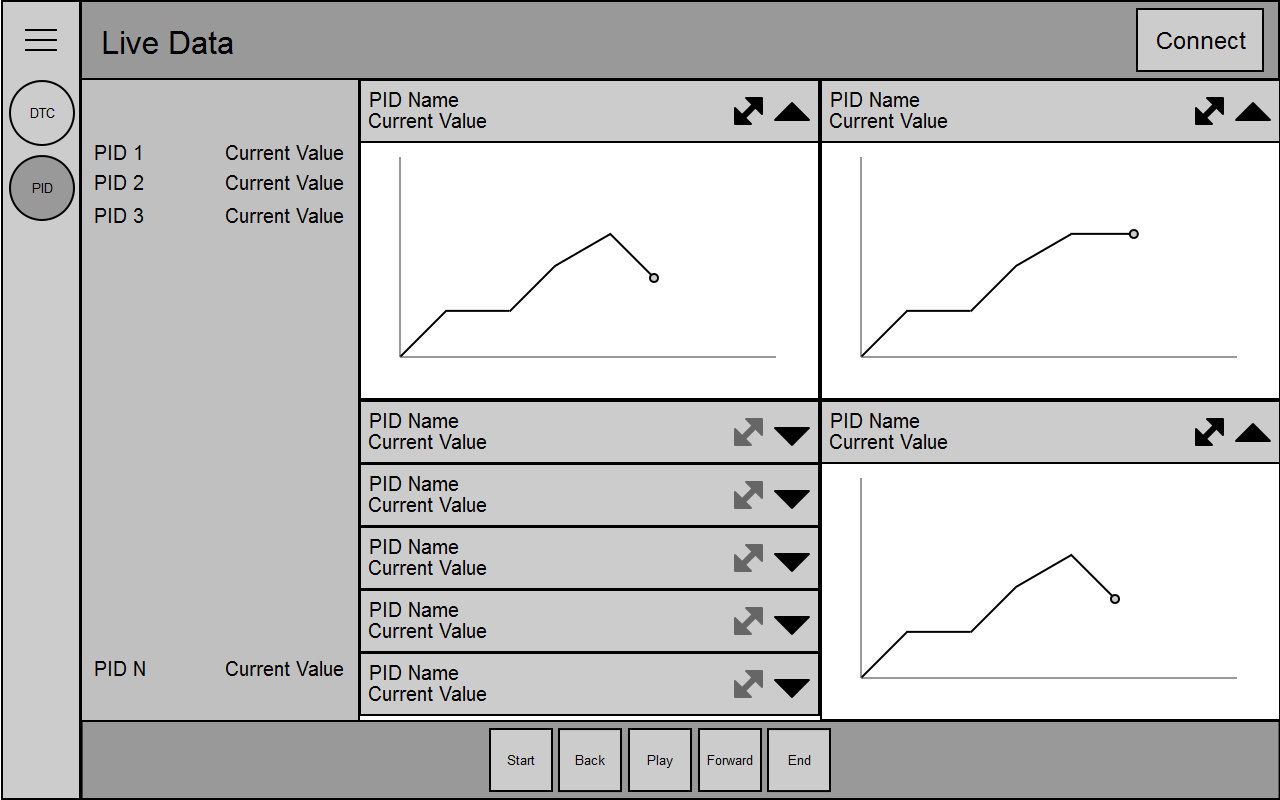
\includegraphics[width=\textwidth]{pidpage2.png}
					\caption{Data Page - Graph Collapsed}						
					\label{fig:DataPage2}
				\end{minipage}									
			\end{center}
		\end{figure}
	
	\newpage
	\subsection{Connection Module}{
		\paragraph{}{
		The user interface for connecting to a device was a key component of the project. As this would be the first thing a user would see on loading the application, it had to provide a suitable amount of information, whilst also being minimalist enough as to not confuse the user. There were two design options considered for this user interface. 
		%[Intro]
		}

		\begin{figure}[h]
			\begin{center}								
				\begin{minipage}{0.49\textwidth}
					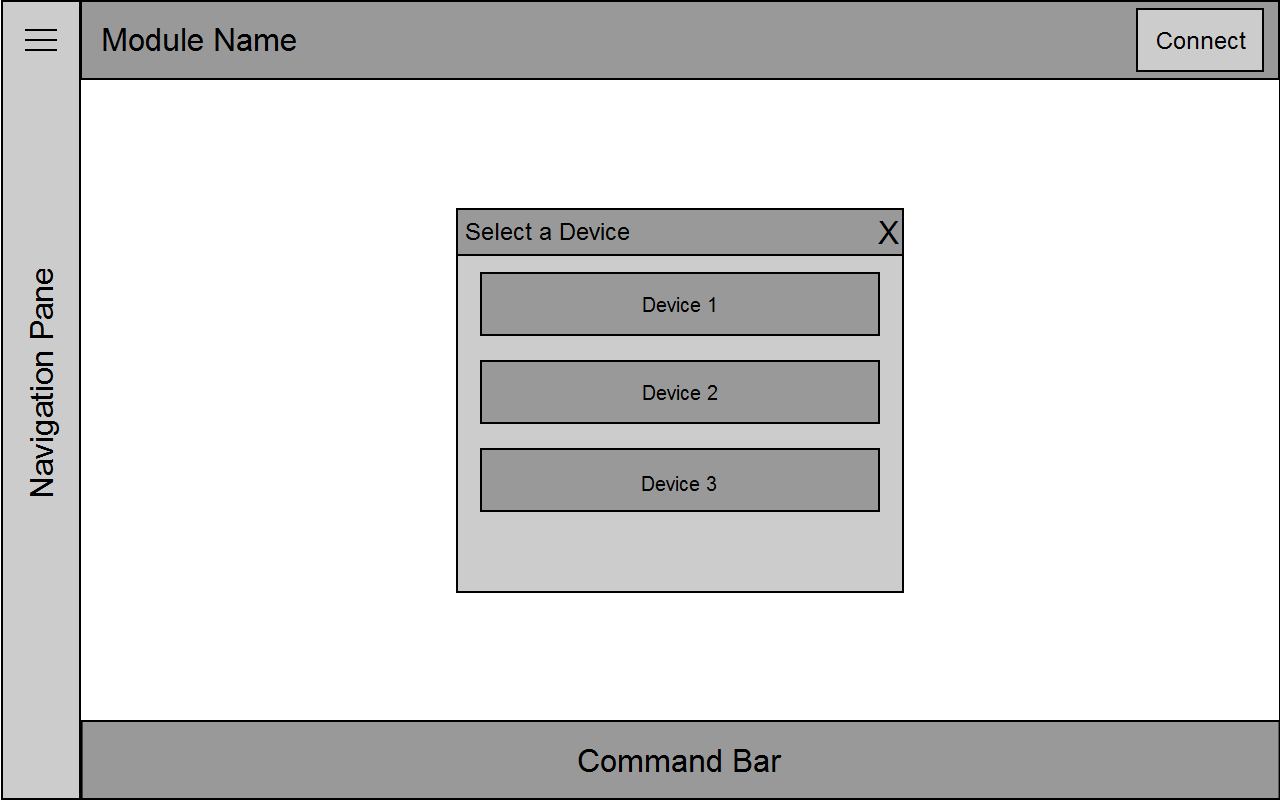
\includegraphics[width=\textwidth]{connectionpage1.png}
					\caption{Connection Design 1}						
					\label{fig:ConnectionPage1}
				\end{minipage}
				\hfill			
				\begin{minipage}{0.49\textwidth}
					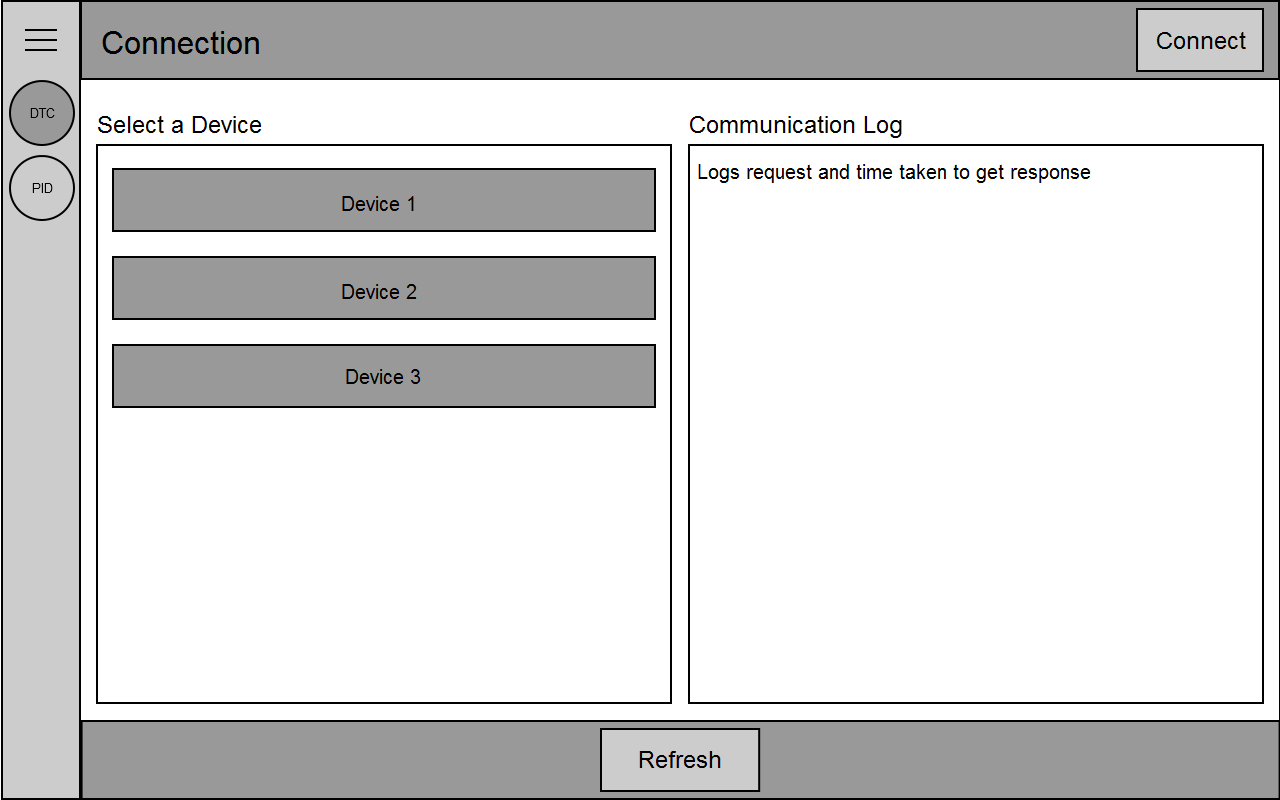
\includegraphics[width=\textwidth]{connectionpage2.png}
					\caption{Connection Design 2}						
					\label{fig:ConnectionPage2}
				\end{minipage}									
			\end{center}
		\end{figure}
		
		\paragraph{}{
		Figure \ref{fig:ConnectionPage1} shows the first design consideration. In this design, a modal box is displayed after clicking the connect button, blocking the user interface behind it. This modal box contains a button for each Bluetooth device paired with the PC. The user can click each button to attempt to connect to the corresponding device. This design is minimalistic and less invasive, as it does not take up a large amount of screen real estate. However, this is also its main drawback, as less space means that only a small amount of instructions can be displayed. As this is the first screen the user will see, they will need to be guided through the setup stages, such as where the ELM327 is connected and how they can pair it to their PC.
		%[Option A]
		}
		
		\paragraph{}{
		Figure \ref{fig:ConnectionPage2} shows the second design consideration. In this design, a module page is created for the connection process. Similar to the first design, the page contains a list of buttons for Bluetooth devices paired to the PC. However, because this design has more screen real estate, a communication log and instructions can be included. The communication log contains information about the communication process, such as any requests that were made and how long it took to receive a response. While this approach allows for more information to be displayed, it requires adding a new module to the existing architecture, so more code is required for this solution.
		%[Option B]
		}
		
		\paragraph{}{
		Ultimately, the second design was used in the final product. While the minimalistic design of the first solution was aesthetically pleasing, it did not match the overall look and feel of the other user interfaces. From a usability perspective, the inclusion of a communication log increased the visibility of the system, allowing a user to see if a request was taking a long time. Overall, the design was selected as it recognised the importance of including instructions on the screen and maintaining a cohesive and visible system.
		%Matched overall deisgn of system, allowed for more information to be displayed to the user on how to connect
		%[Solution]
		}
	}
	\label{ssec:DesignConnectionModule}
	\subsection{Home Module}
		\paragraph{}{
		
		}
